
\section{Evaluation}
\label{sec:evaluation}

This section describes the evaluation process and presents the results of the evaluation.

Evaluation is important because:
\begin{itemize}
  \item It allows us to decide if the quality of the recommender engine archives the desired results.
  \item Evaluation allows us to adjust the parameters in order to get better results.
  \item It allows us to compare different recommender techniques.
\end{itemize}

For recommenders which predict the preferences of a user we can evaluate it by calculating the difference between the estimated preference and the actual preference.
The recommender engine discussed in this article does not estimate preference values in order to produce recommendations. It presents a ordered list of $n$ recommendations. The list is ordered from best to worst recommendation. For this reason we measure the quality of the recommender with precision and recall. Precision and Recall are two information retrieval concepts. We provide a brief summary here to each of these measures.

\subsection{Precision and Recall}
\label{sec:precision}

\begin{description}
\item[Precision] Precision is the proportion of items in the search result that are relevant \cite{Manning}.
  \begin{equation}
    \label{eq:precision}
    \text{Precision} = \frac{\text{number relevant items recommended}}{\text{size of the recommendation list}}
  \end{equation}

 Suppose the recommender create a list of 5 items. If 3 items are relevant recommendations then the precision is $3/5$. 
Precsion only considers the accuracy of the recommendation list and not the comprehensiveness of the result.
\item[Recall] Recall is the proportion of relevant items that appear in the recommendation result. 
  \begin{equation}
    \label{eq:precision}
    \text{Recall} = \frac{\text{number relevant items recommended}}{\text{relevant items}}
  \end{equation}
Suppose there are 9 relevant recommendations. If the recommender results contains 3 of these relevant recommendations then the recall is 3/9.
\end{description}

Listing \ref{lst:irstats} shows the implementation of precision and recall. 
The method \verb|recommender.recommend| returns a list of recommended items for the active user. We check how many items in the recommendation list are also in the list \verb|relevantItemIds| and save the number in \verb|intersectionSize|. 

\begin{lstlisting}[caption=Implementation of precision and recall,label=lst:irstats]
double precision = 0;
double recall = 0;
List<RecommendedItem> recommendedItems = recommender.recommend(userID, howMany);
      for (RecommendedItem recommendedItem : recommendedItems) {
        if (relevantItemIDs.contains(recommendedItem.getItemID())) {
          intersectionSize++;
        }
      }
// Precision
int numRecommendedItems = recommendedItems.size();
if (numRecommendedItems > 0) {
        precision = ((double) intersectionSize / (double) howMany);
      }
// Recall
if (numRecommendedItems > 0) {
 recall =  intersectionSize / (double) numRelevantItems);
      }
\end{lstlisting}

If we want to evaluate a recommender, we have to define, what's a relevant recommendation. Relevancy depends on the goal of the recommender. For example, an item is relevant if the user would give it a high rating or if he would purchase the item.

We define that items which the active user would like or give a high rating are relevant. 
Those ratings are unknown at the time of the recommendation. Nobody knows how a user likes some new item in the future.
But we can simulate the prefencences of the future by setting aside a small part of the real data set as test data. We split the collected input data into two sets.
\begin{itemize}
\item Training data set
\item Test data set
\end{itemize}

We determine the top the top $n$ preferences for each user. Then we remove these values from the input data set. The resulting set is the training data set. We use this set to compute the co-occurence indicator matrix from section \ref{sec:llr}.

The removed entries from the test data set. Items in the test data set are the relevant items. We use this set to compute precision and recall.
For example, if $n$ is 5 this would mean precision is evaluated by removing the top 5 preferences for a user and then finding the percentage of those 5 items included in the top 5 recommendations for that user. 

The evaluatuation of the recommender can be devided into several steps:
\begin{enumerate}
\item  Compute the indicator matrix with the training set.
\item Update the search engine with the similarity values.
\item Generate a list of recommendations $r_u$ for each user.
\item Measure the precision and recall for all generated recommendations list $r$ and return the mean value.
\end{enumerate}

The evaluation process has the following parameters:
\begin{description}
\item[Size of the result] The number of recommendations to consider. The length of the recommendation list.
\item[Relevance threshold] Determines if an item is relevant or not.
\end{description}

\pgfplotsset{width=7cm}
\begin{figure}
  \centering
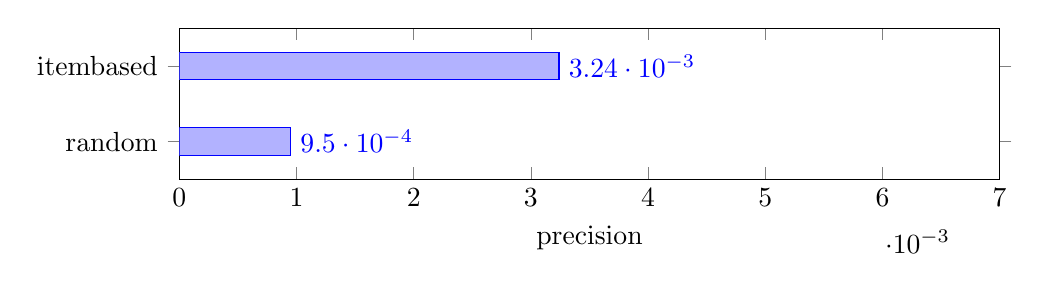
\begin{tikzpicture}
\begin{axis}[
xbar,
xmin=0,
xmax=0.007,
width=12cm,
height=3.5cm,
enlarge y limits=0.5,
xlabel={precision},
symbolic y coords={random, itembased},
ytick=data,
nodes near coords,
nodes near coords align={horizontal},
]

\addplot coordinates {(0.00324,itembased) (0.00095,random)};
\end{axis}
\end{tikzpicture} 
  \caption{Precision and recall comparison of an random generated recommendations and recommendations of itembased recommonder. The number of recommended items is 15}
  \label{fig:precisionrecallvalues}
\end{figure}

In order to get a feel what values of precision an recall to excpect we measured an itembased recommender and random generated recommendion list \cite{jannach11}.
An itembased recommender engine archives an average precision value of 0.00358. This seems a small value but if we return randomly generated recommendations we get a precision of 0.00095. Hence an itembased recommender improves the precision with a factor of 3. Figure \ref{fig:precisionrecallvalues} shows the comparison of the two measurements. We used the movielens data set for this evaluation (see section \ref{sec:dataset}).

\subsection{Dataset}
\label{sec:dataset}

This dataset used in this project describes rating and free-text tagging activity from MovieLens, a movie recommendation service \cite{movielensdata}.
MovieLens data sets were collected by the GroupLens Research Project at the University of Minnesota.
 
This data set consists of:
\begin{itemize}
\item 100,000 ratings. The ratings are numbers from 1 to 5.
\item 943 users. Each user has rated at least 20 movies
\item 1682 movies. Movies are categorized in genres. 
\end{itemize}

The data was collected through the MovieLens web site (movielens.umn.edu) during the seven-month period from September 19th, 1997 through April 22nd, 1998 \cite{movielens}.

All selected users had rated at least 20 movies.
All ratings are contained in the file ratings.csv. Each line of this file after the header row represents one rating of one movie by one user, and has the following format:

\begin{verbatim}
userId,movieId,rating,timestamp.
\end{verbatim}

All tags are contained in the file $tags.csv$. Each line of this file after the header row represents one tag applied to one movie by one user, and has the following format:
\begin{verbatim}
userId,movieId,tag,timestamp
\end{verbatim}

\subsection{Movielens}
\label{sec:movielens}

The MovieLens dataset describes 5-star rating and free-text tagging activity from MovieLens, a movie recommendation service. It contains 100023 ratings and 2488 tag applications across 8570 movies. These data were created by 706 users 

\subsection{Parameters}
\label{sec:parameters}

The recommender has the follwowing parameters:
\begin{itemize}
\item The number of ratings or tags that are used for the query.
\item $n$ the number of items in the result set.
\item Similarity Threshhold. Value that defines if the items shows up in the indicator list of the search engine.
\end{itemize}

\subsection{Baseline Algorithm}
\label{sec:baselinealgorithm}

We compare the co-occurence based recommender to an item-based recommender. This section will give a brief description of item based recommenders.

\subsection{Results}
\label{sec:results}
\begin{figure}
  \centering
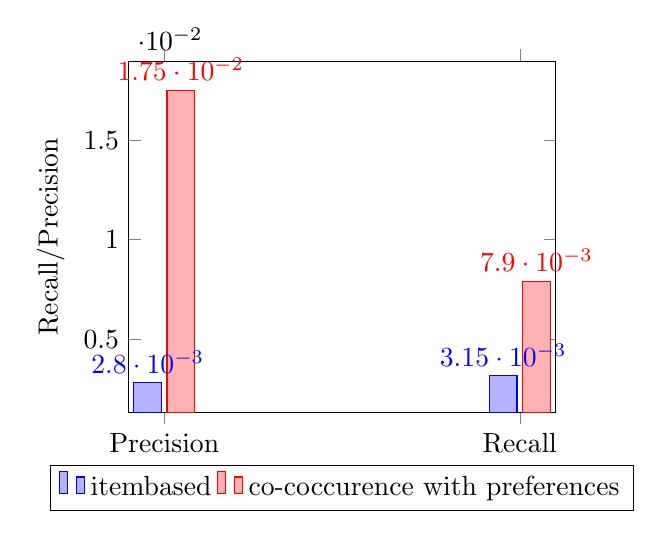
\begin{tikzpicture}
\begin{axis}[
ybar,
%enlargelimits=0.45,
legend style={at={(0.5,-0.15)},
anchor=north,legend columns=-1},
ylabel={Recall/Precision},
symbolic x coords={Precision,Recall},
xtick=data,
%ybar=5pt,% configures ‘bar shift’
%bar width=9pt,
nodes near coords,
nodes near coords align={vertical},
]
\addplot coordinates {(Precision,0.0028) (Recall,0.00315)}; 
\addplot coordinates {(Precision,0.0175) (Recall,0.0079)};

\legend{itembased,co-coccurence with preferences}
\end{axis}
\end{tikzpicture} 
  \caption{Precision and recall comparison of an item-itembased recommonder and the cooccurrence based. The result setsize is 10}
  \label{fig:results}
\end{figure}
